\begin{figure}
	\centering
	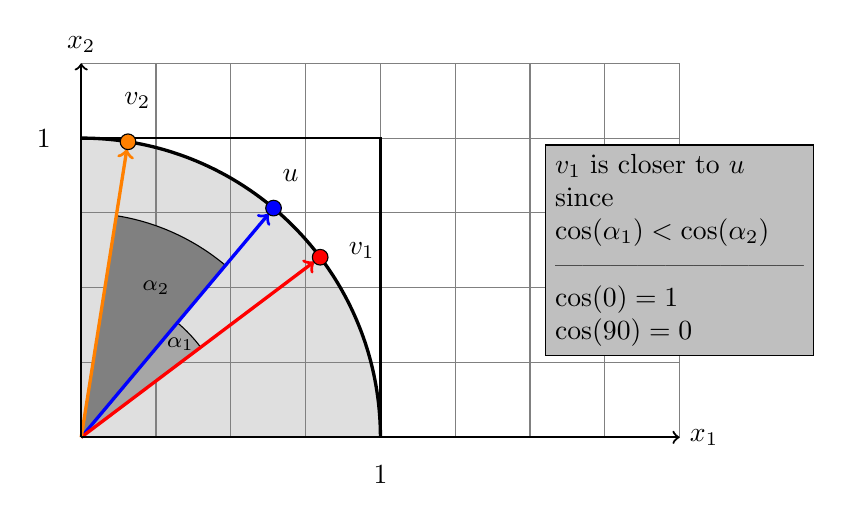
\begin{tikzpicture}[
		scale=0.95
	]

		\fill[lightgray,opacity=0.5] (0,0) -- (4,0) arc[radius=4,start angle=0,end angle=90] -- cycle;
		\draw[gray] (0,0) grid (8,5);
		\draw[thick] (0,4) -- (4,4) -- (4,0);

		\draw[very thick] (0:4) arc[radius=4,start angle=0,end angle=90];

		\fill[gray!70] (0,0) -- (37:2) arc[radius=2,start angle=37,end angle=50] -- cycle;
		\fill[gray] (0,0) -- (50:3) arc[radius=3,start angle=50,end angle=81] -- cycle;

		\draw (37:2) arc[radius=2,start angle=37,end angle=50];
		\draw (50:3) arc[radius=3,start angle=50,end angle=81];
	
		\draw[->,blue,very thick] (0,0) -- (50:3.9);
		\path (0,0) -- (50:4) node[circle,draw=black,fill=blue,inner sep=0.2em] {};
		\draw[->,red,very thick] (0,0) -- (37:3.9);
		\path (0,0) -- (37:4) node[circle,draw=black,fill=red,inner sep=0.2em] {};
		\draw[->,orange,very thick] (0,0) -- (81:3.9);
		\path (0,0) -- (81:4) node[circle,draw=black,fill=orange,inner sep=0.2em] {};

		\node at (1.325,1.25) {\footnotesize{$\alpha_1$}};
		\node at (1,2) {\footnotesize{$\alpha_2$}};

		\node at (2.8,3.5) {$\bm{u}$};
		\node at (3.75,2.5) {$\bm{v}_1$};
		\node at (0.75,4.5) {$\bm{v}_2$};

		\node at (4,-0.5) {1};
		\node at (-0.5,4) {1};

		\node[align=left,black,rectangle,draw=black,fill=lightgray] at (8,2.5) {
			$\bm{v}_1$ is closer to $\bm{u}$ \\
			since \\
			$\cos(\alpha_1) < \cos(\alpha_2)$ \\
			--------------------------- \\
			$\cos(0) = 1$ \\
			$\cos(90) = 0$
		};

		\draw[->,thick] (0,0) -- (8,0) node[right] {$x_1$};
		\draw[->,thick] (0,0) -- (0,5) node[above] {$x_2$};

	\end{tikzpicture}
\end{figure}